\section{Cockroft Walton}\label{ch:cock}
\todo[color=c04x,inline]{testing the colors}
The Cockroft-Walton Multiplier (CWM) utilises passive components to multiply a fluctuating voltage input.
The input voltage does not need to be a pure AC wave,
but also works with any DC shift.
A schematic of the CWM can be seen in Figure \ref{fig:CWM}.

\begin{figure}[H]
   \centering
   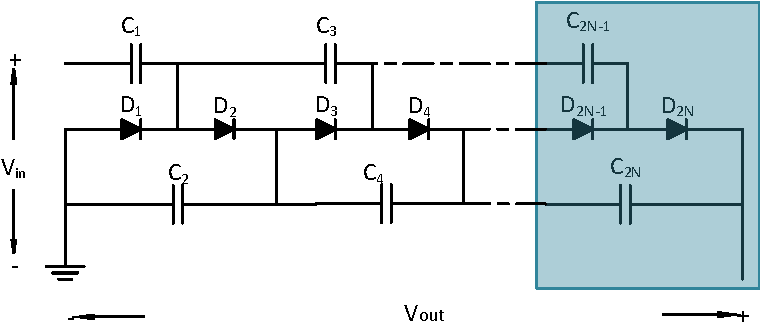
\includegraphics[width=0.6\textwidth]{figures/xCockroftWalton/CockroftWalton.pdf}
    \caption{Schematic of the Cockroft-Walton Multiplier}
	\label{fig:CWM}
\end{figure}

%\subsection{Additions from Conventional BC}
The figure shows a three stage CWM,
with the third stage marked with a blue box.
Since all stages are equal and just appended to the previous,
more stages can be added instead of the dotted lines.

%\subsection{Analysis of Individual Stage}
\begin{figure}[H]%
    \centering
    \subfloat[Negative half Wave\label{sfig:1neg}]{
    	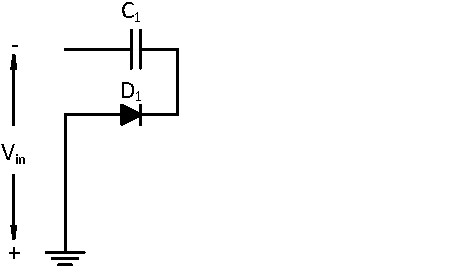
\includegraphics[width=0.45\textwidth]{figures/xCockroftWalton/1neg.pdf}
    }%
    \qquad
    \subfloat[Positive half Wave\label{sfig:2pos}]{
    	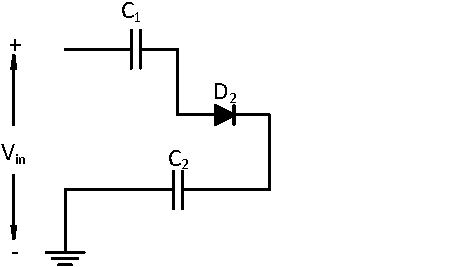
\includegraphics[width=0.45\textwidth]{figures/xCockroftWalton/2pos.pdf}
    }\\%  
    \subfloat[Negative half Wave\label{sfig:3neg}]{
    	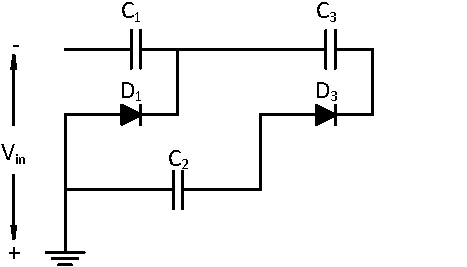
\includegraphics[width=0.45\textwidth]{figures/xCockroftWalton/3neg.pdf}
    }%
    \qquad
    \subfloat[Positive half Wave\label{sfig:4pos}]{
    	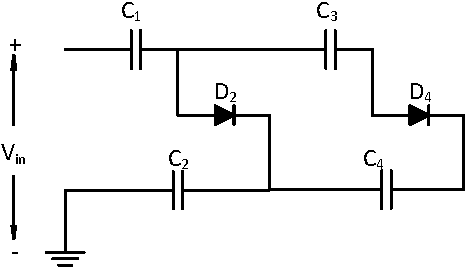
\includegraphics[width=0.45\textwidth]{figures/xCockroftWalton/4pos.pdf}
    }%  
    \caption{CWM Circuit Equivalents for Alternating $V_{in}$}%
    \label{fig:CockBothWave}% 
\end{figure}

Figure \ref{fig:CockBothWave} shows the relevant parts of the CWM circuit at alternating input polarity.
When the upper terminal is negative with respect to ground,
the top capacitors (uneven names) are charged (Subfigures \ref{sfig:1neg} \& \ref{sfig:3neg}).
When the upper terminal is positive with respect to ground,
the bottom capacitors are charged (Subfigures \ref{sfig:2pos} \& \ref{sfig:4pos}).

This behaviour is possible through the placement of the diodes.
Every diode $D_n$ where $n > 1$ is forward biased under the condition shown in Equation \ref{eq:DiodeOnCW}.

\begin{equation}
	V_{C_{n-1}}-V_D \geq V_{C_n}
	\label{eq:DiodeOnCW}
\end{equation}

$C_1$ is charged directly by the input voltage
Equation \ref{eq:DiodeOnCW} therefore also states the voltage across an individual stage dependent on the previous stage,
